\subsection{Parallelisierung}
Zu Beginn unserer Arbeit unterschätzten wir die enorme Datenmenge in Form von Orthofotos (Beispiel Schweiz: 7.1 Millionen Bilder à $5820 m^{2}$ Fläche pro Bild). Weiter wird auch sehr viel Rechenleistung für die Erkennung der Fussgängerstreifen auf den Bilder benötigt. Um diesen nicht trivialen Problemen Herr zu werden, setzten wir auf eine Parallelisierungsstratege mit Hilfe einer Queue. \\ 

\decision{Queueing Sytem}
Den Entscheid für Redis \cite{Redis} in Kombination mit RQ \cite{RQ} haben wir während eines Meeting mit Hilfe von Mitarbeitern des Institut für Software erarbeitet. RQ ist eine relativ einfach zu verwendende Library, welche Redis (Key Value Store) als Queue einsetzt. Durch die Einfachheit und die gute Integration in Python haben wir uns für diesen Lösungsweg entschieden.

\newpage
\subsubsection{Aufbau}
\label{subsec:ablauf}
\begin{figure}[H]
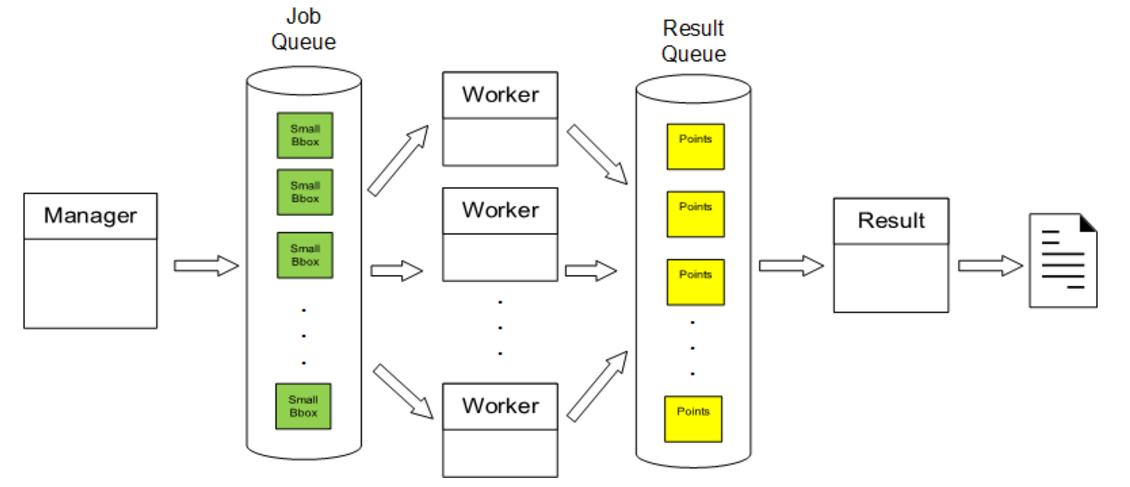
\includegraphics[width=\textwidth]{images/queuing.png}
\caption[Queueing]{Queueing}
\end{figure}
Auf der Abbildung ist zu sehen, dass wir für das Verarbeiten der Jobs auf zwei Queues setzten, eine die die Abzuarbeitenden Bounding Boxes beinhaltet und eine weitere für das Sammeln der Resultate. Der genau Ablauf gestaltet sich wie folgt:
\begin{enumerate}
		\item Manager wird aufgerufen mit der grosse Input Bounding Box.
		\item Manager teilt Bounding Box auf.
		\item Kleine Bounding Boxes werden als Jobs in die Job Queue geladen.
		\item Jobs werden von den Worker aus der Queue geholt.
		\item Worker arbeiten kleine Bounding Boxen ab.
		\item Worker stellt die gefunden Punkt in Result Queue.
		\item Result Worker holt die gefunden Punkt aus der Result Queue und speichert diese in einer JSON Datei ab. 
\end{enumerate}
\newpage









